%%%%%%%%%%%%%%%%%%%%%%%%%%%%%%%%%%%%%%%%%%%%%%%%%%%%%%%%%%%%%%%%%%%%%%%%%%%%%%%%%%%%%%%%%%%%%%%%%%%%%%
% Plantilla básica de Latex en Español.
%
% Autor: Andrés Herrera Poyatos (https://github.com/andreshp)
%
% Es una plantilla básica para redactar documentos. Utiliza el paquete fancyhdr para darle un
% estilo moderno pero serio.
%
% La plantilla se encuentra adaptada al español.
%
%%%%%%%%%%%%%%%%%%%%%%%%%%%%%%%%%%%%%%%%%%%%%%%%%%%%%%%%%%%%%%%%%%%%%%%%%%%%%%%%%%%%%%%%%%%%%%%%%%%%%%

%-----------------------------------------------------------------------------------------------------
%	INCLUSIÓN DE PAQUETES BÁSICOS
%-----------------------------------------------------------------------------------------------------

\documentclass{article}

% Lenguaje
\usepackage[spanish,es-noquoting, es-tabla, es-lcroman]{babel}
\usepackage[utf8]{inputenc}
\selectlanguage{spanish}
\usepackage[colorlinks]{hyperref}

% fuente mono
\usepackage{fontspec}
\setmonofont{Inconsolata}

% Matemáticas
\usepackage{amsthm}
\usepackage{amsfonts}
\usepackage{amsmath}
\usepackage{tikz-cd}
\theoremstyle{plain}
\newtheorem{theorem}{Teorema}
\newtheorem{proposition}{Proposición}
\newtheorem{lemma}{Lema}
\newtheorem{corollary}{Corolario}
\theoremstyle{definition}
\newtheorem{definition}{Definición}
\newtheorem*{axiom}{Axioma}
\theoremstyle{remark}
\newtheorem*{remark}{Nota}
\renewcommand*{\proofname}{Demostración}

\DeclareMathOperator{\Inv}{Inv}
\DeclareMathOperator{\fr}{Fr}
\DeclareMathOperator{\rad}{Rad}
\DeclareMathOperator{\dist}{dist}

\newcommand{\abs}[1]{\ensuremath\left\vert #1 \right\vert}
\newcommand{\norm}[1]{\ensuremath\left\Vert #1 \right\Vert}
\newcommand{\normt}[1]{\ensuremath\left\vert\kern-0.25ex\left\vert\kern-0.25ex\left\vert #1 \right\vert\kern-0.25ex\right\vert\kern-0.25ex\right\vert}

% Corrige el espacio previo a las definiciones
\makeatletter
\def\thm@space@setup{%
  \thm@preskip=\parskip \thm@postskip=0pt
}
\makeatother

% Fuente
\usepackage{courier}
\usepackage{microtype}


% ----
% Estilo de página
%----
% Paquetes para el diseño de página:
\usepackage{fancyhdr}               % Utilizado para hacer títulos propios.
\usepackage{lastpage}               % Referencia a la última página. Utilizado para el pie de página.
\usepackage{extramarks}             % Marcas extras. Utilizado en pie de página y cabecera.
\usepackage[parfill]{parskip}       % Crea una nueva línea entre párrafos.
\usepackage{geometry}               % Asigna la "geometría" de las páginas.

% Se elige el estilo fancy y márgenes de 3 centímetros.
\pagestyle{fancy}
\geometry{left=3cm,right=3cm,top=3cm,bottom=3cm,headheight=1cm,headsep=0.5cm} % Márgenes y cabecera.
\fancyhf{}

% Espacios en el documento:
\linespread{1.1}                        % Espacio entre líneas.
\setlength\parindent{0pt}               % Selecciona la indentación para cada inicio de párrafo.

% Cabecera del documento. Se ajusta la línea de la cabecera.
\renewcommand\headrule{
	\begin{minipage}{1\textwidth}
	    \hrule width \hsize
	\end{minipage}
}

% Texto de la cabecera:
\lhead{\docauthor}                          % Parte izquierda.
\chead{}                                    % Centro.
\rhead{\subject \ - \doctitle}              % Parte derecha.

% Pie de página del documento. Se ajusta la línea del pie de página.
\renewcommand\footrule{
\begin{minipage}{1\textwidth}
    \hrule width \hsize
\end{minipage}\par
}

\lfoot{}                                                 % Parte izquierda.
\cfoot{}                                                 % Centro.
\rfoot{Página\ \thepage\ de\ \protect\pageref{LastPage}} % Parte derecha.


% ----
% PORTADA
% ----

% Estilo
\usepackage{title1}

% Título y autores
\newcommand{\doctitle}{Disco de Poincaré}
\newcommand{\docsubtitle}{}
\newcommand{\docdate}{1 \ de \ Enero \ de \ 2015}
\newcommand{\subject}{Geometría hiperbólica}
\newcommand{\docauthor}{M. Gómez, E.M. González, D. Melero, M. Román}
\newcommand{\docaddress}{Universidad de Granada}
\newcommand{\docemail}{}

% Resumen
\newcommand{\docabstract}{En la geometría hiperbólica, el quinto postulado de Euclides es sustituido por el axioma de Lobachevsky.}

\begin{document}

\maketitle

% Profundidad del Índice
%\setcounter{tocdepth}{1}
\newpage
\tableofcontents
\newpage

\section{Introducción}

La \textbf{geometría hiperbólica} es el modelo axiomático que se
obtiene al aceptar los cuatro primeros postulados de la geometría
euclídea y sustituir el quinto postulado, por el postulado de
Lobachevsky. A pesar de este cambio, algunos aspectos y teoremas
de la geometría euclídea que sean independientes del quinto postulado
seguirán siendo válidos.

Históricamente, se han realizado esfuerzos por deducir el quinto
postulado de Euclides de los otros cuatro. \textit{Giovanni Gerolamo
  Saccheri} intentó, en el siglo XVIII probarlo por reducción al
absurdo y creó en el proceso un modelo incipiente de geometría
hiperbólica que nunca llegó a formalizar en su creencia de que sería
inconsistente. Por otro lado, \textit{Johann Heinrich Lambert} estudió
lo que constituirían los triángulos de la geometría hiperbólica probando
que sus ángulos sumaban siempre menos que 180º. En particular demostró
la fórmula de Lambert para el defecto de un triángulo $T$ de ángulos
$\alpha,\beta,\gamma$ como

\[
  \pi - \alpha- \beta - g = \mathrm{área}(T)k
\]

siendo $k$ una constante de proporcionalidad que estaría relacionada
con la curvatura del espacio hiperbólico. \cite{cedelberg89} Más adelante Carl Friedrich
Gauss trabajaría en un modelo similar sin publicar resultados.

La geometría hiperbólica que conocemos hoy surge en los años 1820
gracias al trabajo independiente de \textit{János Bolyai} y
\textit{Nikolai Ivanovich Lobachevsky}, que publicaron modelos que
posibilitaban una geometría completamente consistente y sin el quinto
postulado. El axioma de Lobachevsky, unido a los cuatro postulados
anteriores, define la geometría hiperbólica.

\begin{axiom}[Axioma de Lobachevsky]
  Dada una recta R y un punto P fuera de R, en el plano conteniendo a
  la línea R y al punto P existen al menos dos líneas distintas que pasan
  por P y no intersecan a R.
\end{axiom}


\section{Modelos de la geometría hiperbólica}
\begin{definition}
  Un \textbf{modelo} para un sistema se define sustituyendo los
  términos indefinidos del sistema de axiomas por objetos específicos
  que los cumplen.
\end{definition}

Por ejemplo, un modelo de la geometría euclídea es el que asigna a
cada punto un par de reales $(a,b)$ y a cada recta el conjunto de
puntos que satisfacen una ecuación lineal $as+bt+u = 0$ para algunos
reales tales que al menos uno de ellos no sea $0$. Existen varios
modelos de geometría hiperbólica:

\begin{itemize}
  
\item la \textbf{representación de Klein}, también conocida como el
  \textit{modelo proyectivo del disco} o \textit{modelo de
    Beltrami-Klein}, toma como puntos a los puntos interiores de
  un círculo en el plano euclídeo y como rectas a las cuerdaas del
  círculo.
  
\item el \textbf{modelo del disco de Poincaré}, usa también el
  interior de un círculo plano unidad como espacio de puntos,
  pero toma como rectas los arcos de circunferencia que cortan el
  borde del círculo plano de forma ortogonal.
  
\item el \textbf{modelo del hiperboloide} o \textit{de Lorentz} usa
  como espacio de puntos una hoja de un hiperboloide de dos hojas
  y como rectas los cortes de este con los hiperplanos del espacio
  de Minkowski en el que se embebe el hiperboloide.
  
\end{itemize}

Aunque los dos primeros fueron publicados por \textit{Eugenio
  Beltrami} en 1968, se hicieron conocidos por el uso que les
darían \textit{Felix Klein} y \textit{Henri Poincaré}. Ambos
son modelos que estudiaremos en su caso bidimensional pero
generalizables a más dimensiones.

\subsection{Modelo del hiperboloide}

El \textbf{modelo del hiperboloide} de la geometría hiperbólica se
basa en la forma cuadrática de Lorentz,
\[L(x,y,z)=x^2+y^2-z^2.\]

Si pensamos en esta forma cuadrática como una norma, tendremos vectores
distintos de cero con norma cero e incluso norma negativa. Esto nos da
una clasificación de los vectores en

\begin{enumerate}
\item vectores espaciales, $x\in\mathbb{R}^3$ tales que $L(x)>0$;
\item vectores temporales, $x\in\mathbb{R}^3$ tales que $L(x)<0$; y
\item vectores luminosos, $x\in\mathbb{R}^3$ tales que $L(x)=0$.
\end{enumerate}

Con esta norma definimos
\[\mathbb{H}^2=\{(x,y,z)\in\mathbb{R}^3 \mid L(x,y,z)=-1,\; (x,y,z) \cdot (0,0,1) > 0 \};\]
y como vemos, esta es la hoja superior de un hiperboloide de dos
hojas. Sabemos que es una superficie y por tanto localmente
homeomorfo a un plano, por lo que lo llamaremos \textit{plano hiperbólico}.

\begin{itemize}
\item Los puntos en $\mathbb{H}$ serán los puntos de nuestro modelo
  de la geometría hiperbólica.
\item Las rectas en el plano hiperbólico se definen como las intersecciones
  de $\mathbb{H}$ con planos que pasan por el origen. Las llamaremos
  \textit{rectas hiperbólicas}.
\end{itemize}



\subsection{Disco de Poincaré}

\subsubsection{Métrica en el disco de Poincaré}
Si $u,v$ son dos vectores del espacio euclídeo $\mathbb{R}^n$,ambos
con norma inferior a $1$, podemos definir un invariante isométrico de
la siguiente manera:
\[\delta (u,v)=2\frac{\norm{u-v}^2}{(1-\norm{u}^2)(1-\norm{v}^2)},\]

donde $\norm{.}$ representa la norma euclídea usual. Definimos la
función distancia como:
\[d(u,v)=arccosh(1+\delta(u,v)).\]

Esta función de distancia está definida para cualesquiera dos vectores
de norma inferior a uno, y el conjunto de tales vectores forman un
espacio métrico que es un modelo de espacio hiperbólico de curvatura
constante $-1$, como sabemos el disco de Poincaré.

La función $\operatorname{arccosh}$ es creciente, luego cuanto mayor
sea $\delta(u,v)$, mayor será la distancia que separa $u$ y $v$. Ahora
bien, si acercamos uno de los dos vectores $u$ o $v$ hacia la frontera
del disco, su norma se acercará a uno, la función $\delta$ crecerá, y
como consecuencia la función distancia también. Es decir, si tenemos
dos vectores, uno suficientemente lejos de la frontera y vamos
acercando el otro a la frontera, la distancia entre ambos crecerá.

Por ejemplo, en la siguiente imagen todos los puntos están a la misma
distancia del punto $A$:

\begin{figure}[h]
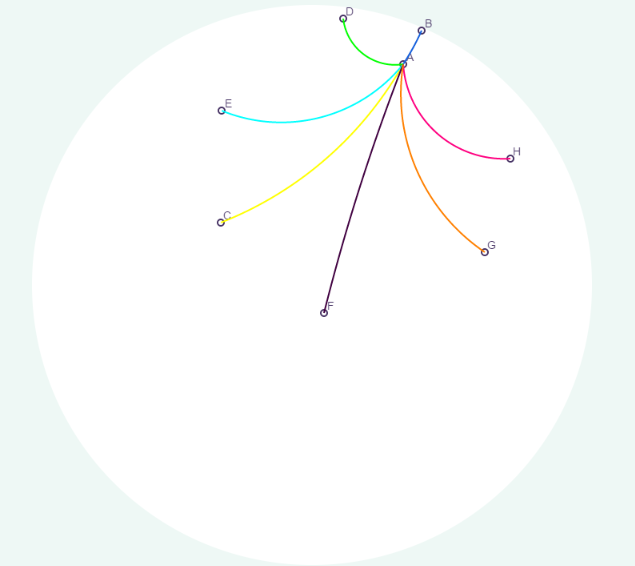
\includegraphics{Distancias.png}
\end{figure}

Veamos también como sería una circunferencia con centro $A$ un punto
cercano a la frontera y de radio, por ejemplo, 4:

\begin{figure}[h]
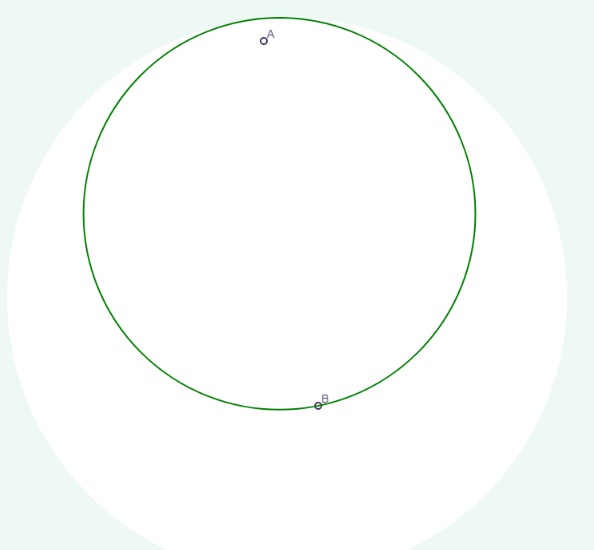
\includegraphics{Circunferencia.png}
\end{figure}


\subsubsection{Rectas}

Dados ahora dos puntos vamos a ver como es la recta que pase por los
dos puntos dados. En el modelo del disco de Poincaré, las rectas del
plano se definen por arcos de circunferencias con ecuaciones de la
forma
\[x^2+y^2+ax+by+1=0,\]
que es la forma general de una circunferencia que corta ortogonalmente al disco unidad.\\
Dados dos puntos $u$ y $v$ en el disco que no estén en un diámetro, se
puede resolver para el círculo de esta forma pasando por ambos puntos,
y obtener
$$x^{2}+y^{2}+{\frac {u_{2}(v_{1}^{2}+v_{2}^{2})-v_{2}(u_{1}^{2}+u_{2}^{2})+u_{2}-v_{2}}{u_{1}v_{2}-u_{2}v_{1}}}x+{\frac {v_{1}(u_{1}^{2}+u_{2}^{2})-u_{1}(v_{1}^{2}+v_{2}^{2})+v_{1}-u_{1}}{u_{1}v_{2}-u_{2}v_{1}}}y+1=0.$$

\subsubsection{Ángulos}
Los ángulos son euclidianos. Si tenemos dos líneas hiperbólicas, cada
una de ellas es un arco de circunferencia, luego la medida del ángulo
que se forma entre las dos líneas hiperbólicas es el ángulo que forman
las tangentes de las circunferencias en el punto en que éstas se
intersecan.

\subsubsection{Relación con el modelo del hiperboloide}
Este modelo se relaciona con el modelo del hiperboloide
proyectivamente. Dado un punto $(t, x_1,x_2)$ sobre la hoja superior
de un hiperboloide del modelo del hiperboloide, se define un punto del
modelo del disco de Poincaré, que se puede proyectar sobre el plano
t=0,el resultado es el correspondiente punto del disco de Poincaré.
Para las coordenadas cartesianas $(t,x_1,x_2)$ del hiperboloide e
$(y_1,y_2)$ del plano, las fórmulas de conversión son :

\[
  y_{i}=\frac {x_{i}}{1+t}
  \qquad
  (t,x_{i})=\frac {(1+\sum {y_{i}^{2}},2y_{i})}{1-\sum {y_{i}^{2}}}
\]


\section{Construcciones en el espacio hiperbólico}
\subsection{Cuadriláteros de Saccheri}
\begin{definition}
  Un \textbf{cuadrilátero de Saccheri} es un cuadrilátero $ABCD$ con
  dos ángulos rectos adyacentes en $A$ y $B$ y con dos lados iguales
  $\overline{AD} = \overline{BC}$.
\end{definition}

Nótese que en el plano hiperbólico no podemos demostrar de la misma
forma que lo hacíamos en el plano euclídeo que los ángulos en $C$ y
$D$ sean rectos. De hecho, si lo fueran, podríamos deducir el quinto
postulado. A pesar de esto, sí podemos demostrar que son iguales.

\begin{theorem}
  En un cuadrilátero de Saccheri, los dos ángulos no rectos son
  iguales.
\end{theorem}

Y además, podemos demostrar que la base del cuadrilátero es ultraparalela
con su lado opuesto.

\begin{theorem}
  La línea que une los puntos medios de la base del cuadrilátero de
  Saccheri y su opuesto corta a ambas perpendicularmente. De aquí se
  sigue que ambas son ultraparalelas.
\end{theorem}

\subsection{Círculos y horociclos}
Sabemos ya que dos rectas distintas en el espacio hiperbólico
deben ser secantes, paralelas o ultraparalelas. Deberán por tanto
pertenecer a uno de los siguientes conjuntos

\begin{itemize}
\item un \textbf{haz} de todas las rectas que pasan por un punto.
\item un \textbf{haz de paralelas} con todas las rectas paralelas a un
  rayo dado.
\item un \textbf{haz de ultraparalelas} con todas las líneas
  perpendiculares a una línea dada.
\end{itemize}

Usaremos las reflexiones sobre estas rotaciones para caracterizar los
círculos y definir con ellas los horociclos por analogía con la
caracterización y los hiperciclos por analogía con la definición.

\begin{definition}[Círculo]
  Dado un punto $C$ y un radio $r \geq 0$, llamamos \textbf{círculo}
  al conjunto de puntos a distancia $r$ de él, es decir,
  \[{\cal C} = \left\{ X \mid \mathrm{dist}(X,C) = r \right\}.\]
\end{definition}

\begin{theorem}
  Un círculo con centro $O$ puede construirse como la órbita de un punto
  sobre las reflexiones que determina el haz de rectas que pasa por $O$.
\end{theorem}

\begin{definition}[Horociclo]
  Dado un haz de rectas paralelas a un rayo, definimos un \textbf{horociclo} como
  la órbita de un punto $C$ bajo las reflexiones determinadas por las rectas del
  haz. \cite{coxeter}
\end{definition}

Podemos interpretar un horociclo como un círculo teniendo como centro un
punto impropio en el infinito.

\begin{definition}[Hiperciclo]
  Llamamos \textbf{hiperciclo} al lugar geométrico dado por los puntos a
  una distancia fija de una recta.
\end{definition}

Podemos caracterizarlo a su vez como la órbita de un punto bajo las reflexiones
sobre las rectas de un haz de ultraparalelas.\cite{coxeter}

\subsection{Polígonos}
\begin{theorem}
  Los ángulos constructibles en el plano euclídeo son exactamente los ángulos
  constructibles en el plano hiperbólico. \cite{jagy95}
\end{theorem}

En particular, podemos construir un hexágono regular en el plano
hiperbólico, que tiene todos sus lados y ángulos iguales, como puede
apreciarse en la figura \ref{hexagon}. Nótese que el área dependerá de
sus ángulos, por lo que podremos construir en particular hexágonos con
todos sus ángulos rectos

\begin{figure}[ht!]
\centering
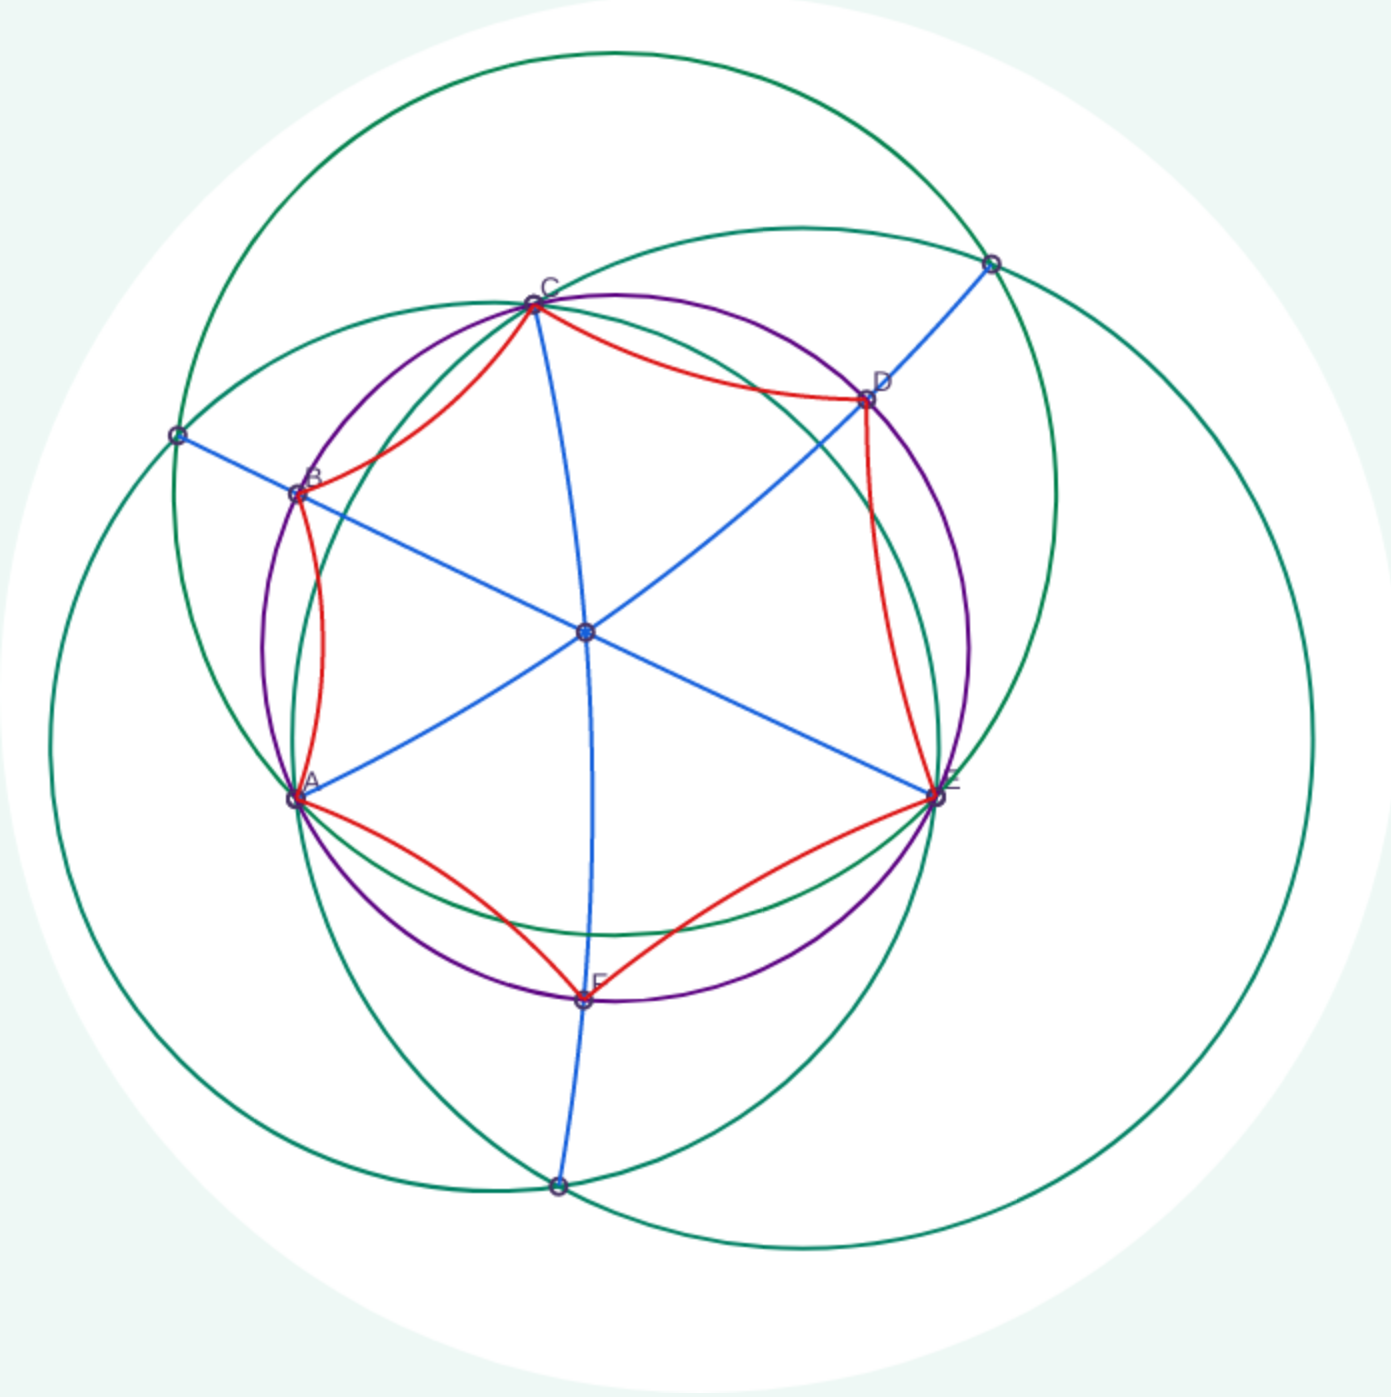
\includegraphics[width=90mm]{./hexagon.png}
\caption{Construcción del hexágono regular \label{hexagon}}
\end{figure}

\subsection{Teselaciones}
\subsubsection{Teselación con hexágonos rectos}
Podemos teselar un plano hiperbólico con hexágonos con todos sus ángulos rectos,
como puede apreciarse en la figura \ref{teselahexagon}.
Nótese que todos ellos son \textit{congruentes}.

\begin{figure}[ht!]
  \centering
  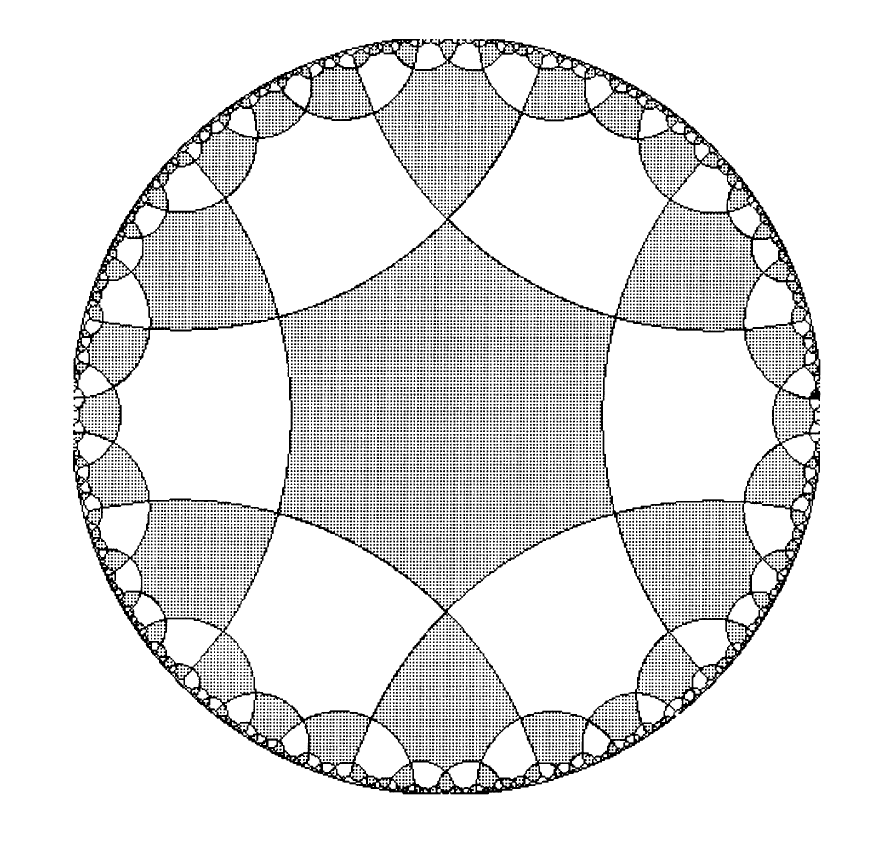
\includegraphics[width=80mm]{./teselahexagonos.png}
  \caption{Teselación con hexágonos rectos\label{teselahexagon}}
\end{figure}


% https://www.rose-hulman.edu/mathjournal/archives/2014/vol15-n1/paper2/v15n1-2pd.pdf

\section{Construcciones interactivas}
Enumeramos a continuación varias implementaciones de construcciones interactivas
con regla y compás hiperbólicos en un disco de Poincaré.

\subsection{NonEuclid}
\textbf{NonEuclid} es una aplicación ligera permitiendo construcciones
con regla y compás en un disco de Poincaré e interactividad con las
construcciones, además de soporte simple para animaciones. La versión
original fue escrita en Java en 1994 por Joel Castellanos, pero en
2016 se implementó una versión en Javascript que puede ejecutarse
desde el navegador usando HTML5. El código de ambas es abierto (si
bien no consta de licencias de software libre), y puede obtenerse en
la página web de
\href{https://www.cs.unm.edu/~joel/NonEuclid/NonEuclid.html}{NonEuclid}.

Para este trabajo hemos alojado una instancia de NonEuclid en la
página que indica \href{https://m42.github.io/hiperboloide/}{este
  enlace} y hemos aportado construcciones nuevas a las originalmente
seleccionables por la aplicación.

\subsection{Geogebra}
\textbf{Geogebra} no soporta directamente las construcciones en geometría
hiperbólica, pero la comunidad aporta hojas de trabajo particulares en las
que están presentes herramientas de construcción para varios modelos del
plano huperbólico en licencia Creative Commons. Un ejemplo es
\href{https://www.geogebra.org/material/show/id/2028857}{esta construcción}
de Francis W. Lipinski, sobre la que hemos realizado construcciones menores.

\subsection{Cinderella}
\textbf{Cinderella} es software propietario escrito en Java que soporta geometrías
euclídea, esférica e hiperbólica.

\section{Referencias}
\begin{thebibliography}{9}

\bibitem{cedelerg89}
  Judith N. Cedelberg (1989-2001),
  A Course in Modern Geometries,
  New York: Springer Science and Business Media.

\bibitem{singer98}
  David A. Singer (1998),
  Geometry: Plane and Fancy,
  New York: Springer Science and Business Media.

\bibitem{ryan}
  Patrick J. Ryan
  Euclidean and non euclidean geometry. An analytic approach.

\bibitem{coxeter}
  Wiley; Coxeter,
  Introduction to Geometry.

\bibitem{jagy95}
  William Jagy (1995),
  Squaring Circles in the Hyperbolic Plane,
  The Mathematical Intelligencer.
  
\end{thebibliography}

\end{document}
